% !TeX spellcheck = fr_FR
\chapter{Chapitre 2 : Historique du projet}

\section{Projet initial}

En novembre 2023, l'\gls{unige} a proposé ce projet de recherche à l'\gls{hepia}, spécifiquement dans le cadre du projet du télescope spatial Terzina. 
Le but initial de ce projet était de créer un modèle de machine learning permettant d'aider à la décision d'événements scientifiquement intéressant 
détecté par le télescope afin de réduire la quantité d'informations a transmettre au sol. 
Le télescope Terzina est prévu d'être lancé à bord du satellite NUSES.

\subsection{NUSES}
Le projet \textbf{NeUtrino and Seismic Electromagnetic Signals} est une mission spatiale pionnière qui 
a vu le jour via la collaboration entre différentes universités et organisations gouvernementales. \cite{Nuses}
Notamment l'\gls{unige}, l'\gls{infn} et la NASA.
Son but est d'envoyer un satellite dans l'espace, avec deux instruments scientifiques à bord, Zirè et Terzina, qui mènerons 
des expériences une fois en orbite.

\begin{figure}[tbph!]
	\centering
	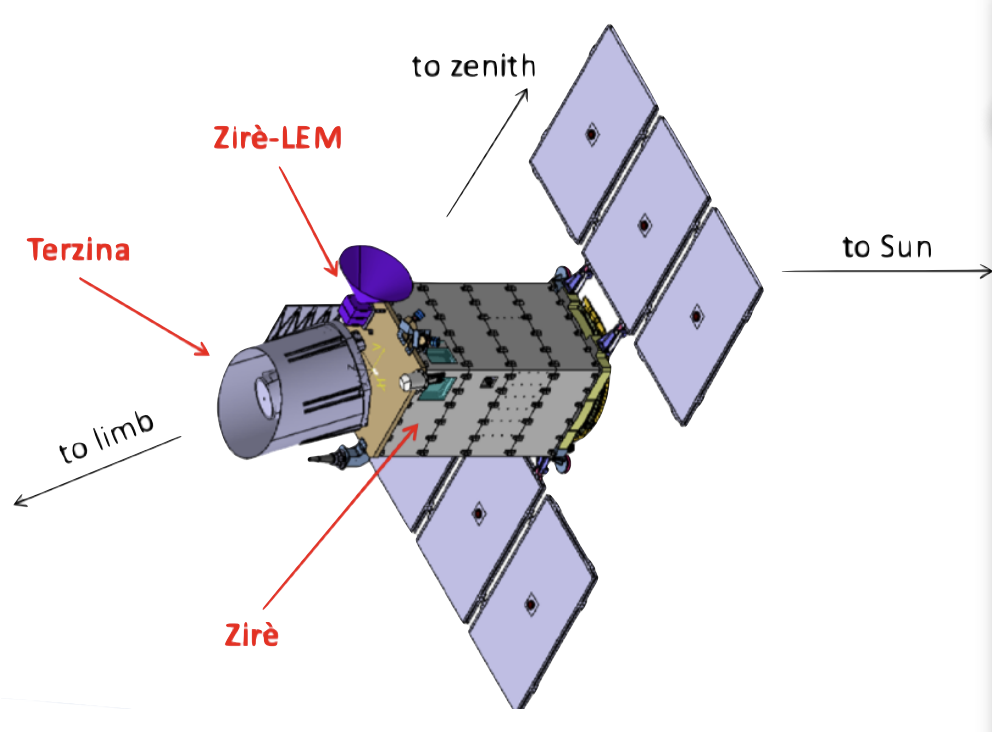
\includegraphics[width=0.7\linewidth]{nuses.png}
	\caption[Mission NUSES]{Mission NUSES. Source: \cite{Nuses}}
\end{figure}

\textbf{Zirè} a pour but d'observer le rayonnement cosmique \gls{le} (<250 MeV) pour étudier de plus près la ceinture de Van Allen,
la météo spatiale et les interactions entre les lithosphère, ionosphère et magnétosphère.

\textbf{Terzina} a pour but de tester de manière concrète les technologies qui pourraient être utilisées pour étudier des rayonnements cosmiques
\gls{uhe} > 100PeV et de détecter des neutrinos via les pluies atmosphériques de lumière Cherenkov qu'ils produisent.

%comparaison with the Japanese detector in mountains ?

Le satellite sera placé en orbite terrestre basse de manière héliosynchrone.
L'orbite terrestre basse ou \gls{leo} est définie comme toutes les orbites plus proches que 1000km au dessus de la surface de la terre.\cite{LowEarthOrbit}
L'orbite héliosynchrone est une orbite presque polaire (naviguant du nord au sud ou inversement) où le satellite 
passe au dessus d'un même point à la même heure solaire. Cela implique que son orientation en rapport au soleil reste la même.

Pour Terzina, cela permet aux capteurs d'être toujours pointés en direction opposée au soleil pour éviter au maximum les rayons gamma qu'il émet.

\begin{figure}[tbph!]
	\centering
	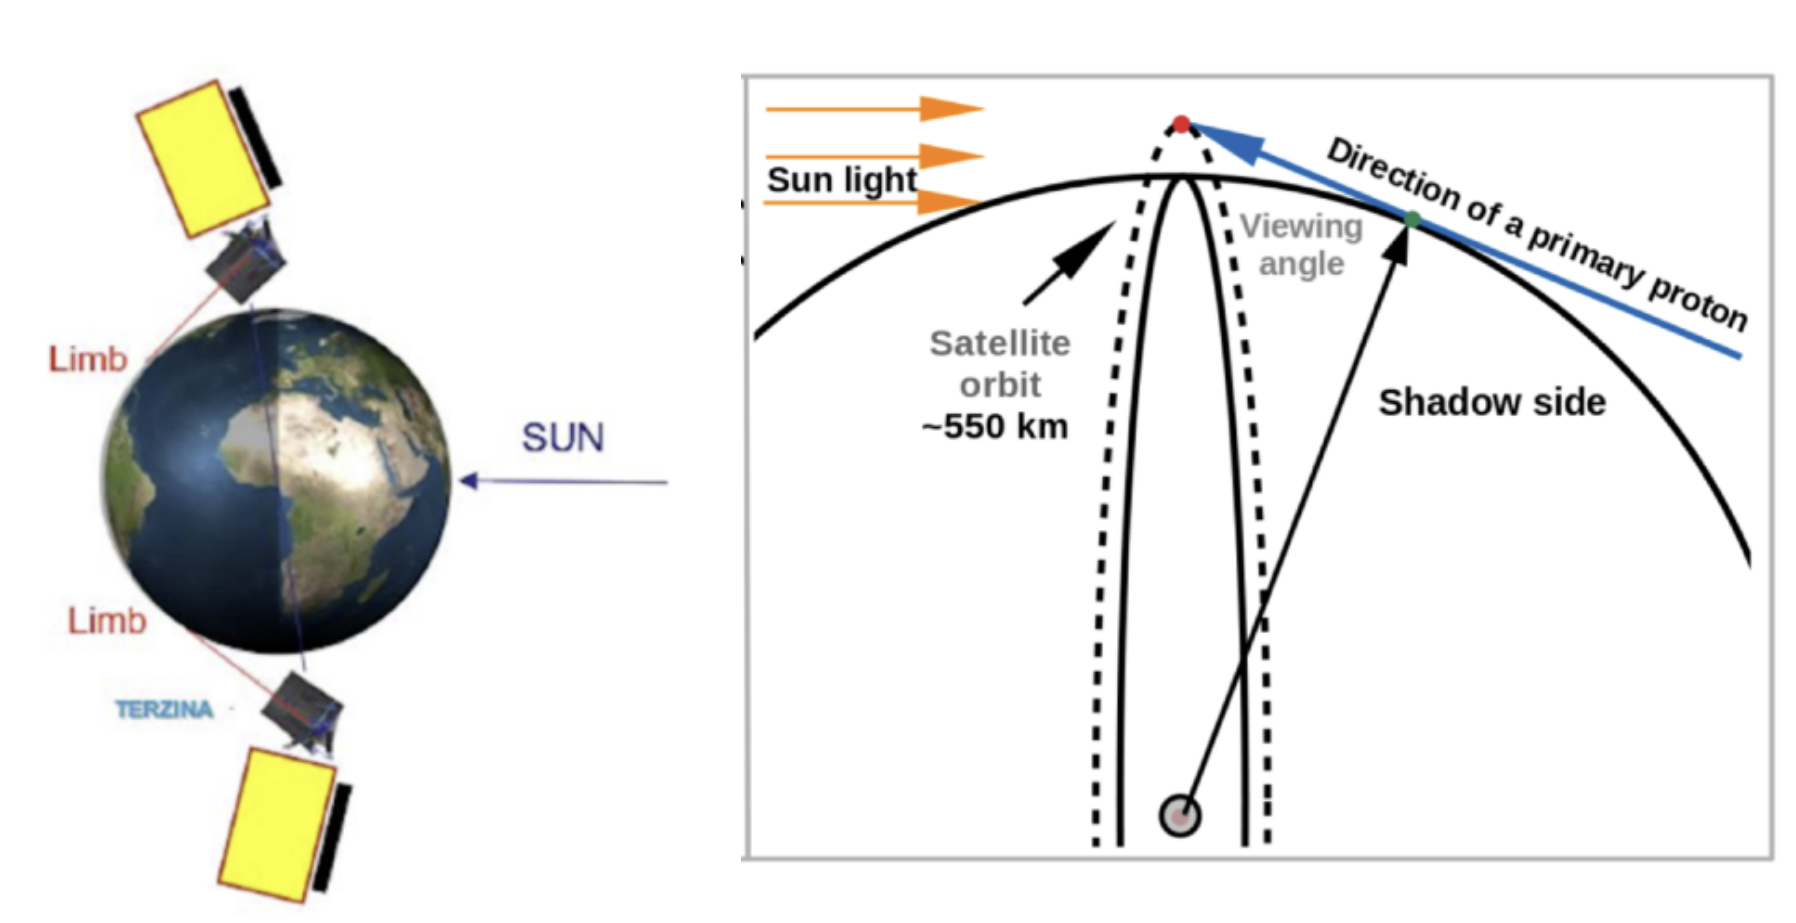
\includegraphics[width=0.7\linewidth]{heliosynchrone.png}
	\caption[Orbite héliosynchrone de Terzina]{Orbite héliosynchrone de Terzina. Source: \cite{Nuses}}
\end{figure}

\subsection{Terzina}
Comparé aux autres satellites qui ont étudiés des rayons gamma en orbite, Terzina est prévu d'être le premier télescope spatial
qui détectera la lumière Cherenkov depuis l'espace. De plus, il permettra aussi d'étudier les performances de nouveaux capteurs \gls{sipm}
dans l'espace. Ceux-ci devraient détecter plus de photons et être plus robustes que leur contrepartie classique bien que ces nouveaux capteurs
soient plus sensible aux bruits de fond et à l'irradiation abondante hors de notre atmosphère.

\begin{figure}[tbph!]
	\centering
	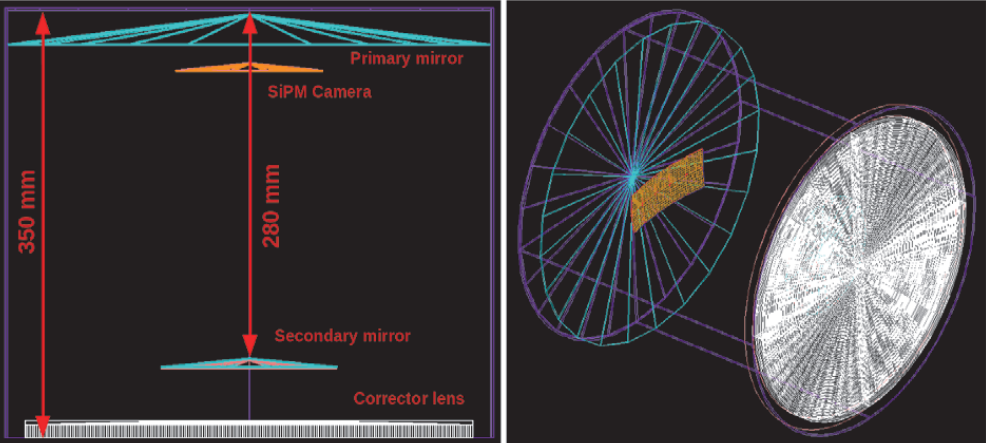
\includegraphics[width=0.7\linewidth]{terzina_mirrors.png}
	\caption[Vue de la configuration optique de Terzina]
	{En bleu les miroirs, en blanc la lentille, en orange la caméra et en violet les murs \textbf{Gauche :} Vue de dessus. \textbf{Droite :} Vue de côté. Source: \cite{Burmistrov_2023} p.2}
\end{figure}

Le télescope utilise une configuration à deux miroirs qui redirigent et concentrent les photons reçus sur une matrice 
rectangulaire de 10 modules \gls{sipm}, eux-mêmes possédant une résolution de 8x8 pixels, 640 pixels au total. \cite{Burmistrov_2023}

Cette forme rectangulaire a été décidée pour observer le limbe terrestre de manière optimale et elle est capable de détecter une coupe transversale de 140 x 360 $km^2$.
Derrière les 10 modules \gls{sipm}, il est prévu 10 \gls{asic} chacun possédant 64 canaux pour chacun des tubes photomultiplicateurs de la caméra.
Ces \gls{asic} sont conçus pour amplifier le signal de sortie puis le numériser avant d'être collectés par un \gls{fpga} à bord du satellite. 

En plus de leur rôle de numérisation, les \gls{asic} ont aussi le rôle de déclencheur matériel. 
Ce rôle est important pour que le signal analogue des photomultiplicateurs ne soit converti en signal numérique que si nécessaire. 

Le premier mécanisme de déclanchement, nommé "haut", arrive lorsque un pic d'énergie dépasse un seuil "haut" dans un seul canal
d'un module \gls{sipm}; chaque canal du module est numérisé et collecté par le \gls{fpga}. 

Le deuxième mécanisme de déclanchement "bas" arrive lorsque deux pixels adjacents d'un même module \gls{sipm}
dépassent ce seuil ou lorsque c'est l'un des 8 pixels voisins d'un autre module. 
Ensuite, les pixels voisins sont analysés pour déterminer si au moins deux d'entre eux ont aussi dépassé ce seuil "bas"; dans ce cas l'\gls{fpga} va conserver cet évènement.
Tous ces tests se déroulent dans un laps de temps très court; de la numérisation du signal au traitement et stockage sur le \gls{fpga}, il se passerait environ 51.2$\mu$s

\section{Proposition de projet par l'UNIGE}

La quantité de données récoltées par Terzina se révèle être trop importante pour être envoyée au sol, même après l'activation des déclancheurs intégrés au matériel.
En effet, la capacité de bande passante de Terzina est limitée à 40Gbit par jour en transmission et seulement quelques Kbit par jour en réception.
Ceci est dû à la configuration du satellite NUSES qui est aussi partagé entre les deux instruments Zirè et Terzina.

C'est à ce moment de la conception que l'UNIGE a eu l'idée d'ajouter un réseau de neurones à bord du \gls{fpga}, capable de filtrer
le bruit de chaque pixel pour n'en garder que les photons de pluies atmosphériques. 
Avec ce signal filtré, la décision d'envoyer ou non l'événement au sol serait plus simple. 
Ils ont donc proposé ce projet à l'\gls{hepia} et j'ai été choisi pour travailler dessus comme projet de semestre.

Les ressources à bord du satellite étant coûteuses, le modèle avait comme contrainte d'être le plus petit possible 
afin d'utiliser le moins de place et de puissance de calcul.
Il est prévu d'utiliser un modèle Keras pour le réseau de neurones, car il existe déjà des moyens de l'exporter vers des \gls{fpga}.
Le déploiement du modèle de réseau de neurones ne faisait pas partie intégrante de ce travail de semestre mais impliquait une
restriction technique car la programmation du \gls{fpga} n'aurait été possible qu'avant le lancement.

En plus de cette utilisation en tant que filtre, l'équipe de l'\gls{unige} a théorisé l'idée que le réseau de neurones
pourrait aussi compenser l'usure et l'irradiation des capteurs au fil du temps. Cette compensation pourrait se faire par un ajustement en vol 
des poids du réseau de neurones ou implicitement par l'architecture et l'entraînement du modèle directement.

\section{Délais de production}

Malheureusement, en mars 2023, l'équipe s'occupant du développement des \gls{asic} à annoncé des retards de production conséquents ne permettant pas de les installer sur Terzina.
Il a donc été décidé de remplacer ces \gls{asic} par un modèle déjà existant : CITIROC. Cependant, ces nouveaux \gls{asic} ne sont pas capables 
de transmettre un signal comme les \gls{asic} prévus jusqu'à présent et ne donnent que des informations sur le pic d'intensité atteint sur la durée d'échantillonage.

% TODO numeric waveform signal vs Peak and time diagram

Ce changement de matériel modifie les données en sortie du capteur, ne produisant plus de signal numérisé et rendant donc la capabilité d'un réseau de neurones
difficile voir impossible.

\section{Adaptation du projet}

Voyant que l'ajout du réseau de neurones sur le \gls{fpga} du télescope n'est plus possible, l'\gls{unige} propose alors de poursuivre 
ce projet de recherche mais pour utilisation sur des télescopes au sol. L'équipe de l'\gls{unige} participe également au groupe \gls{ctao}
qui a pour but de créer deux observatoires dotés de trois types de télescopes différents.

Le réseau de neurones imaginé pour Terzina serait aussi utile pour ces télescopes.
Les télescopes standard ne présentent pas les mêmes contraintes que la légèreté et la simplicité que Terzina doit respecter pour arriver en orbite.
Sans ces contraintes, le \gls{lst} atteint une résolution de $1'855$ pixels et une fréquence d'acquisition de $1 GHz$. 
Cette configuration, collecte $24 Gbit$ de données par seconde avant les systèmes de déclancheurs matériels. \cite{LSTSpecifications}
De plus, la nouvelle génération de caméra sur laquelle l'\gls{unige} travaille, augmentera même la résolution jusqu'à $~8'000$ pixels.

L'ajout d'un réseau de neurones capable de réduire le bruit et d'estimer le nombre de photons détectés par pixel serait donc très utile en tant que 
point de décision supplémentaire pour garder ou non les diférents événements déclanchés afin de réduire les ressources utilisées pour le stockage 
et le traitement de ces données.

De plus, il a été théorisé que le filtrage et l'estimation du nombre de photons que le réseau de neurones apporterait, puissent améliorer 
le traitement des données en aval. Cela pourrait notamment améliorer la résolution angulaire (d'où provient la pluie de lumière Cherenkov) et une possible amélioration de
la sensibilité du télescope aux évènements moins énergétiques.

Pour tester l'amélioration de ces performances, il est prévu d'insérer ce réseau neuronal en tant qu'étape de pré-traitement des données
au pour chaque pixel avant de les transmettre à un logiciel de classification et d'analyse des pluies Cherenkov : CTLearn.

Mais pour sa possible utilisation finale, ce réseau pourrait aussi être programmé dans des \gls{asic} ou \gls{fpga} qui seraient intégrés dans les différents télescopes au sol.

\subsection{CTLearn}
Cet outil, développé en coordination entre l'université de genève et de Madrid, permet d'analyser des pluies Cherenkov détectées 
par les télescopes du \gls{ctao}. CTLearn va alors, pour chaque pluie essayer d'en déterminer son type : hadronique ou électromangnétique, 
sa provenance dans le ciel et effectuer des analyses sur l'énergie totale de cet évènement.
Ces différentes informations sont ensuites utilisées par d'autres projets pour calculer d'autres valeurs d'intérêts scientifiques.

\subsubsection{Data levels}
Pour faciliter la communication et les échanges entre les nombreuses équipes travaillant pour le \gls{ctao}, 
plusieurs niveaux de données ont été élaborés.

\begin{figure}[tbph!]
	\centering
	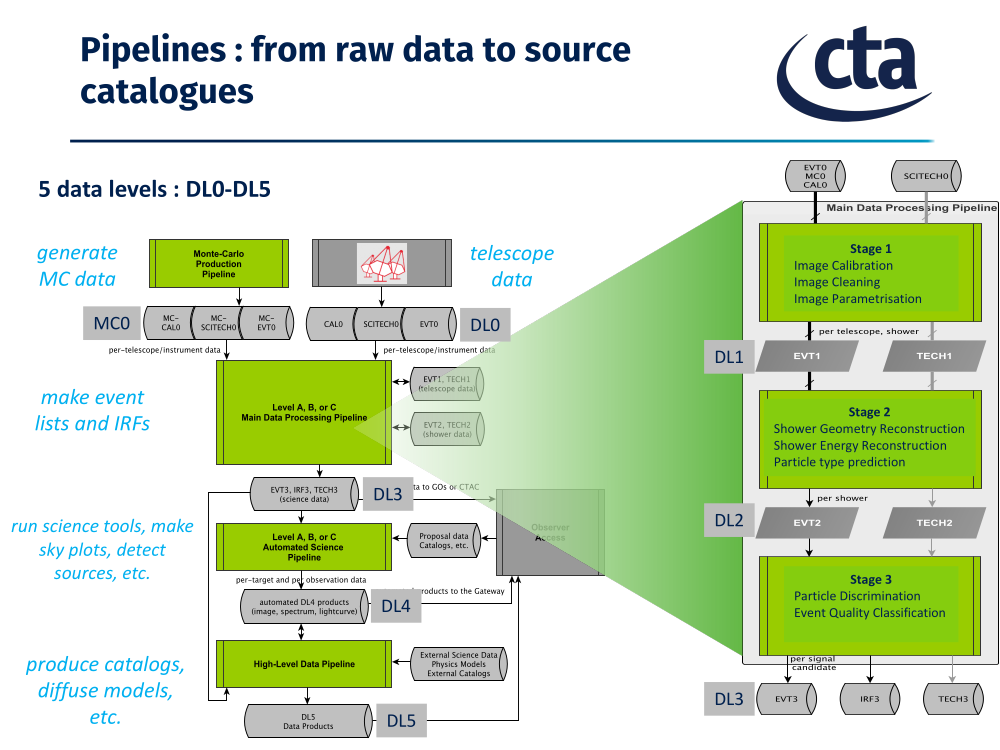
\includegraphics[width=\linewidth]{CTADataLevels.png}
	\caption[Flux des données CTAO]{Flux des données CTAO. Source: \cite{CTAOComputingChallenges}, page 5}
\end{figure}

\begin{itemize}
	\item MC0 : Données créées par des simulateurs Monte-Carlo
	\item DL0 : Données réelles récupérées par les télescopes.
	\item DL1 : Images calibrées et nétoyées (par télescope/pluie Cherenkov)
	\item DL2 : Reconstruction de la pluie selon les images récupérées et prédiction de type hadronique/électromagnétique
	\item DL3 : Qualification et dicrimination des pluies
	\item DL4 : Analyse des données de haut-niveau (spectres du ciel complet, etc.)
	\item DL5 : Aggrégation des données pour en créer des catalogues en tirer des conclusions scientifiques.
\end{itemize}

\subsubsection{Flux logiciel}

\begin{figure}[tbph!]
	\centering
	\includegraphics[width=\linewidth]{CTLearnWorkflow.png}
	\caption[Flux du logiciel CTLearn]{Flux du logiciel CTLearn. Source: \cite{CTLearnWorkflow}}
\end{figure}

Les données utilisées par CTLearn sont les signaux numérisées de chaque capteur composant la caméra d'un télescope, données de niveau DL1.
Ces données sont récupérées via les outils CTAPipe et DL1-Data-Handler. 
Ce projet de bachelor résiderait donc entre DL1-Data-Handler et CTLearn ou serait intégré à l'un d'entre eux comme étape de pré-traitement des signaux individuels.